\documentclass[twoside]{book}

% Packages required by doxygen
\usepackage{fixltx2e}
\usepackage{calc}
\usepackage{doxygen}
\usepackage[export]{adjustbox} % also loads graphicx
\usepackage{graphicx}
\usepackage[utf8]{inputenc}
\usepackage{makeidx}
\usepackage{multicol}
\usepackage{multirow}
\PassOptionsToPackage{warn}{textcomp}
\usepackage{textcomp}
\usepackage[nointegrals]{wasysym}
\usepackage[table]{xcolor}

% Font selection
\usepackage[T1]{fontenc}
\usepackage[scaled=.90]{helvet}
\usepackage{courier}
\usepackage{amssymb}
\usepackage{sectsty}
\renewcommand{\familydefault}{\sfdefault}
\allsectionsfont{%
  \fontseries{bc}\selectfont%
  \color{darkgray}%
}
\renewcommand{\DoxyLabelFont}{%
  \fontseries{bc}\selectfont%
  \color{darkgray}%
}
\newcommand{\+}{\discretionary{\mbox{\scriptsize$\hookleftarrow$}}{}{}}

% Page & text layout
\usepackage{geometry}
\geometry{%
  a4paper,%
  top=2.5cm,%
  bottom=2.5cm,%
  left=2.5cm,%
  right=2.5cm%
}
\tolerance=750
\hfuzz=15pt
\hbadness=750
\setlength{\emergencystretch}{15pt}
\setlength{\parindent}{0cm}
\setlength{\parskip}{3ex plus 2ex minus 2ex}
\makeatletter
\renewcommand{\paragraph}{%
  \@startsection{paragraph}{4}{0ex}{-1.0ex}{1.0ex}{%
    \normalfont\normalsize\bfseries\SS@parafont%
  }%
}
\renewcommand{\subparagraph}{%
  \@startsection{subparagraph}{5}{0ex}{-1.0ex}{1.0ex}{%
    \normalfont\normalsize\bfseries\SS@subparafont%
  }%
}
\makeatother

% Headers & footers
\usepackage{fancyhdr}
\pagestyle{fancyplain}
\fancyhead[LE]{\fancyplain{}{\bfseries\thepage}}
\fancyhead[CE]{\fancyplain{}{}}
\fancyhead[RE]{\fancyplain{}{\bfseries\leftmark}}
\fancyhead[LO]{\fancyplain{}{\bfseries\rightmark}}
\fancyhead[CO]{\fancyplain{}{}}
\fancyhead[RO]{\fancyplain{}{\bfseries\thepage}}
\fancyfoot[LE]{\fancyplain{}{}}
\fancyfoot[CE]{\fancyplain{}{}}
\fancyfoot[RE]{\fancyplain{}{\bfseries\scriptsize Generated by Doxygen }}
\fancyfoot[LO]{\fancyplain{}{\bfseries\scriptsize Generated by Doxygen }}
\fancyfoot[CO]{\fancyplain{}{}}
\fancyfoot[RO]{\fancyplain{}{}}
\renewcommand{\footrulewidth}{0.4pt}
\renewcommand{\chaptermark}[1]{%
  \markboth{#1}{}%
}
\renewcommand{\sectionmark}[1]{%
  \markright{\thesection\ #1}%
}

% Indices & bibliography
\usepackage{natbib}
\usepackage[titles]{tocloft}
\setcounter{tocdepth}{3}
\setcounter{secnumdepth}{5}
\makeindex

% Hyperlinks (required, but should be loaded last)
\usepackage{ifpdf}
\ifpdf
  \usepackage[pdftex,pagebackref=true]{hyperref}
\else
  \usepackage[ps2pdf,pagebackref=true]{hyperref}
\fi
\hypersetup{%
  colorlinks=true,%
  linkcolor=blue,%
  citecolor=blue,%
  unicode%
}

% Custom commands
\newcommand{\clearemptydoublepage}{%
  \newpage{\pagestyle{empty}\cleardoublepage}%
}

\usepackage{caption}
\captionsetup{labelsep=space,justification=centering,font={bf},singlelinecheck=off,skip=4pt,position=top}

%===== C O N T E N T S =====

\begin{document}

% Titlepage & ToC
\hypersetup{pageanchor=false,
             bookmarksnumbered=true,
             pdfencoding=unicode
            }
\pagenumbering{roman}
\begin{titlepage}
\vspace*{7cm}
\begin{center}%
{\Large Ashesi Lab Repository \\[1ex]\large 1.\+0 }\\
\vspace*{1cm}
{\large Generated by Doxygen 1.8.11}\\
\end{center}
\end{titlepage}
\clearemptydoublepage
\tableofcontents
\clearemptydoublepage
\pagenumbering{arabic}
\hypersetup{pageanchor=true}

%--- Begin generated contents ---
\chapter{Hierarchical Index}
\section{Class Hierarchy}
This inheritance list is sorted roughly, but not completely, alphabetically\+:\begin{DoxyCompactList}
\item \contentsline{section}{adb}{\pageref{classadb}}{}
\begin{DoxyCompactList}
\item \contentsline{section}{Booking}{\pageref{class_booking}}{}
\item \contentsline{section}{Equipment}{\pageref{class_equipment}}{}
\end{DoxyCompactList}
\end{DoxyCompactList}

\chapter{Data Structure Index}
\section{Data Structures}
Here are the data structures with brief descriptions\+:\begin{DoxyCompactList}
\item\contentsline{section}{\hyperlink{classadb}{adb} }{\pageref{classadb}}{}
\item\contentsline{section}{\hyperlink{class_booking}{Booking} }{\pageref{class_booking}}{}
\item\contentsline{section}{\hyperlink{class_equipment}{Equipment} }{\pageref{class_equipment}}{}
\end{DoxyCompactList}

\chapter{Data Structure Documentation}
\hypertarget{classadb}{}\section{adb Class Reference}
\label{classadb}\index{adb@{adb}}
Inheritance diagram for adb\+:\begin{figure}[H]
\begin{center}
\leavevmode
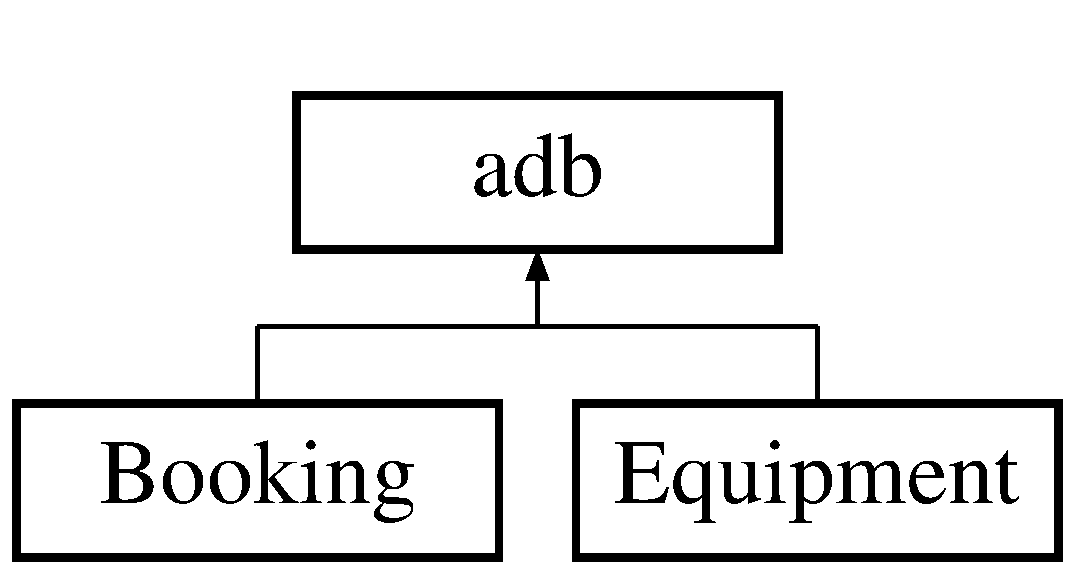
\includegraphics[height=2.000000cm]{classadb}
\end{center}
\end{figure}
\subsection*{Public Member Functions}
\begin{DoxyCompactItemize}
\item 
{\bfseries adb} ()\hypertarget{classadb_a0ec94bd1d566c9082e1a611c3a1621c1}{}\label{classadb_a0ec94bd1d566c9082e1a611c3a1621c1}

\item 
\hyperlink{classadb_a78572828d11dcdf2a498497d9001d557}{connect} ()
\item 
\hyperlink{classadb_a453053eefc3e4a7f1e9931650d0faf33}{query} (\$str\+Query)
\item 
{\bfseries fetch} ()\hypertarget{classadb_ae48cc10bd727774bb36203986ce3b176}{}\label{classadb_ae48cc10bd727774bb36203986ce3b176}

\end{DoxyCompactItemize}
\subsection*{Data Fields}
\begin{DoxyCompactItemize}
\item 
{\bfseries \$db} =null\hypertarget{classadb_a1fa3127fc82f96b1436d871ef02be319}{}\label{classadb_a1fa3127fc82f96b1436d871ef02be319}

\item 
{\bfseries \$result} =null\hypertarget{classadb_a112ef069ddc0454086e3d1e6d8d55d07}{}\label{classadb_a112ef069ddc0454086e3d1e6d8d55d07}

\end{DoxyCompactItemize}


\subsection{Detailed Description}
Database connection helper Database connection helper class 

Definition at line 10 of file adb.\+php.



\subsection{Member Function Documentation}
\index{adb@{adb}!connect@{connect}}
\index{connect@{connect}!adb@{adb}}
\subsubsection[{\texorpdfstring{connect()}{connect()}}]{\setlength{\rightskip}{0pt plus 5cm}connect (
\begin{DoxyParamCaption}
{}
\end{DoxyParamCaption}
)}\hypertarget{classadb_a78572828d11dcdf2a498497d9001d557}{}\label{classadb_a78572828d11dcdf2a498497d9001d557}
Connect to database \begin{DoxyReturn}{Returns}
boolean ture if connected else false 
\end{DoxyReturn}


Definition at line 19 of file adb.\+php.

\index{adb@{adb}!query@{query}}
\index{query@{query}!adb@{adb}}
\subsubsection[{\texorpdfstring{query(\$str\+Query)}{query($strQuery)}}]{\setlength{\rightskip}{0pt plus 5cm}query (
\begin{DoxyParamCaption}
\item[{}]{\$str\+Query}
\end{DoxyParamCaption}
)}\hypertarget{classadb_a453053eefc3e4a7f1e9931650d0faf33}{}\label{classadb_a453053eefc3e4a7f1e9931650d0faf33}
Query the database 
\begin{DoxyParams}[1]{Parameters}
string & {\em \$str\+Query} & sql string to execute \\
\hline
\end{DoxyParams}


Definition at line 34 of file adb.\+php.



The documentation for this class was generated from the following file\+:\begin{DoxyCompactItemize}
\item 
C\+:/xampp/htdocs/projimp1/src/adb.\+php\end{DoxyCompactItemize}

\hypertarget{class_booking}{}\section{Booking Class Reference}
\label{class_booking}\index{Booking@{Booking}}
Inheritance diagram for Booking\+:\begin{figure}[H]
\begin{center}
\leavevmode
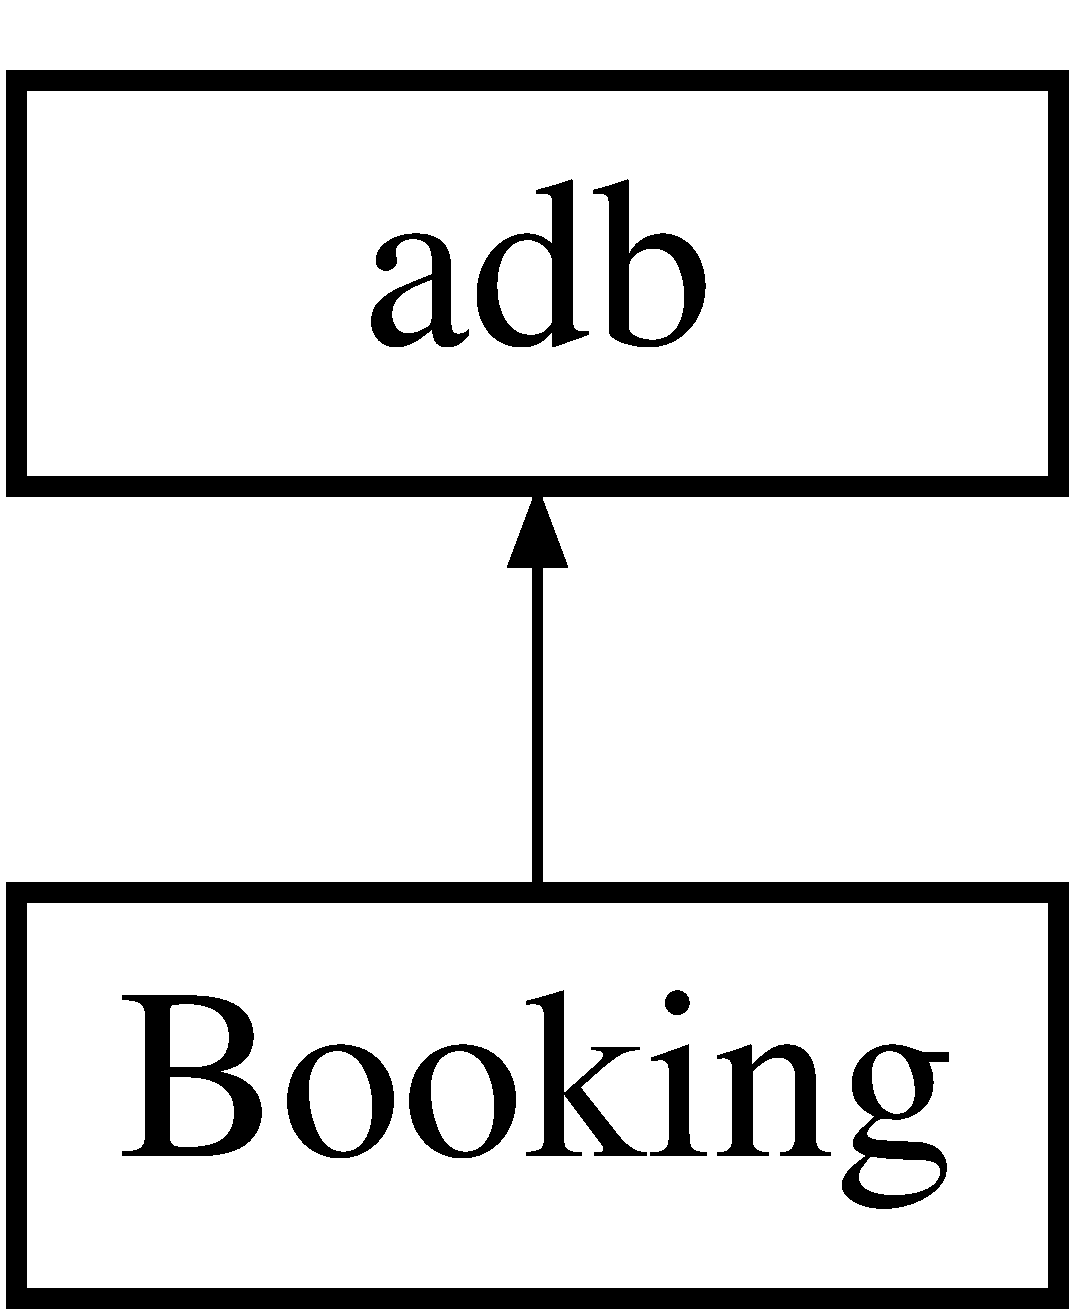
\includegraphics[height=2.000000cm]{class_booking}
\end{center}
\end{figure}
\subsection*{Public Member Functions}
\begin{DoxyCompactItemize}
\item 
{\bfseries Booking} ()\hypertarget{class_booking_a1e9a6bc6b4531385afaa068510394c10}{}\label{class_booking_a1e9a6bc6b4531385afaa068510394c10}

\item 
\hyperlink{class_booking_a926356c5cf1148e86b384c975e979a70}{add\+Booking} (\$Equip\+\_\+\+Id, \$User\+\_\+\+Id)
\item 
\hyperlink{class_booking_a4a891c8631da9e436cbfa3dc5a1af870}{search\+Bookings} (\$Equip\+Name)
\item 
\hyperlink{class_booking_a53c9c60dc2d5200976f52594175dc1eb}{unbook\+Equipment} (\$Booking\+\_\+\+Id)
\item 
\hyperlink{class_booking_ab79fef06fab5b9b19312651cf8ad79f5}{release\+Equip} (\$Equip\+\_\+\+Id)
\item 
{\bfseries book\+Equip} (\$Equip\+\_\+\+Id)\hypertarget{class_booking_a0fd3d89691c5f2391a7fa082ceb8cd01}{}\label{class_booking_a0fd3d89691c5f2391a7fa082ceb8cd01}

\item 
\hyperlink{class_booking_a3dba7af3ac89f0c7c191024c2bcbf2e5}{get\+Bookings} ()
\end{DoxyCompactItemize}
\subsection*{Additional Inherited Members}


\subsection{Detailed Description}
\hyperlink{class_booking}{Booking} class 

Definition at line 8 of file Booking.\+php.



\subsection{Member Function Documentation}
\index{Booking@{Booking}!add\+Booking@{add\+Booking}}
\index{add\+Booking@{add\+Booking}!Booking@{Booking}}
\subsubsection[{\texorpdfstring{add\+Booking(\$\+Equip\+\_\+\+Id, \$\+User\+\_\+\+Id)}{addBooking($Equip_Id, $User_Id)}}]{\setlength{\rightskip}{0pt plus 5cm}add\+Booking (
\begin{DoxyParamCaption}
\item[{}]{\$\+Equip\+\_\+\+Id, }
\item[{}]{\$\+User\+\_\+\+Id}
\end{DoxyParamCaption}
)}\hypertarget{class_booking_a926356c5cf1148e86b384c975e979a70}{}\label{class_booking_a926356c5cf1148e86b384c975e979a70}
Adds a new booking 
\begin{DoxyParams}{Parameters}
{\em int} & Equip\+Id ID of equipment \\
\hline
{\em timestamp} & time\+Booked timestamp of the moment equipment was booked by a user \\
\hline
{\em int} & User\+\_\+\+Id ID of student who booked equipment \\
\hline
\end{DoxyParams}
\begin{DoxyReturn}{Returns}
boolean returns true if successful or false 
\end{DoxyReturn}


Definition at line 24 of file Booking.\+php.

\index{Booking@{Booking}!get\+Bookings@{get\+Bookings}}
\index{get\+Bookings@{get\+Bookings}!Booking@{Booking}}
\subsubsection[{\texorpdfstring{get\+Bookings()}{getBookings()}}]{\setlength{\rightskip}{0pt plus 5cm}get\+Bookings (
\begin{DoxyParamCaption}
{}
\end{DoxyParamCaption}
)}\hypertarget{class_booking_a3dba7af3ac89f0c7c191024c2bcbf2e5}{}\label{class_booking_a3dba7af3ac89f0c7c191024c2bcbf2e5}
method to fetch for all bookings in the system \begin{DoxyReturn}{Returns}
boolean returns true if successful or false 
\end{DoxyReturn}


Definition at line 100 of file Booking.\+php.

\index{Booking@{Booking}!release\+Equip@{release\+Equip}}
\index{release\+Equip@{release\+Equip}!Booking@{Booking}}
\subsubsection[{\texorpdfstring{release\+Equip(\$\+Equip\+\_\+\+Id)}{releaseEquip($Equip_Id)}}]{\setlength{\rightskip}{0pt plus 5cm}release\+Equip (
\begin{DoxyParamCaption}
\item[{}]{\$\+Equip\+\_\+\+Id}
\end{DoxyParamCaption}
)}\hypertarget{class_booking_ab79fef06fab5b9b19312651cf8ad79f5}{}\label{class_booking_ab79fef06fab5b9b19312651cf8ad79f5}
method to cgange the status of an equipment to avaiilable 
\begin{DoxyParams}{Parameters}
{\em int} & Equip\+\_\+\+Id ID of an equipment \\
\hline
\end{DoxyParams}
\begin{DoxyReturn}{Returns}
boolean returns true if successful or false 
\end{DoxyReturn}
method to change the status of an equipment to reserved 
\begin{DoxyParams}{Parameters}
{\em int} & Equip\+\_\+\+Id ID of an equipment \\
\hline
\end{DoxyParams}
\begin{DoxyReturn}{Returns}
boolean returns true if successful or false
\end{DoxyReturn}


Definition at line 72 of file Booking.\+php.

\index{Booking@{Booking}!search\+Bookings@{search\+Bookings}}
\index{search\+Bookings@{search\+Bookings}!Booking@{Booking}}
\subsubsection[{\texorpdfstring{search\+Bookings(\$\+Equip\+Name)}{searchBookings($EquipName)}}]{\setlength{\rightskip}{0pt plus 5cm}search\+Bookings (
\begin{DoxyParamCaption}
\item[{}]{\$\+Equip\+Name}
\end{DoxyParamCaption}
)}\hypertarget{class_booking_a4a891c8631da9e436cbfa3dc5a1af870}{}\label{class_booking_a4a891c8631da9e436cbfa3dc5a1af870}
method to search for bookings related to an equipment with a particular name 
\begin{DoxyParams}{Parameters}
{\em String} & Equip\+Name equipment name you want to search for \\
\hline
\end{DoxyParams}
\begin{DoxyReturn}{Returns}
boolean returns true if successful or false 
\end{DoxyReturn}


Definition at line 41 of file Booking.\+php.

\index{Booking@{Booking}!unbook\+Equipment@{unbook\+Equipment}}
\index{unbook\+Equipment@{unbook\+Equipment}!Booking@{Booking}}
\subsubsection[{\texorpdfstring{unbook\+Equipment(\$\+Booking\+\_\+\+Id)}{unbookEquipment($Booking_Id)}}]{\setlength{\rightskip}{0pt plus 5cm}unbook\+Equipment (
\begin{DoxyParamCaption}
\item[{}]{\$\+Booking\+\_\+\+Id}
\end{DoxyParamCaption}
)}\hypertarget{class_booking_a53c9c60dc2d5200976f52594175dc1eb}{}\label{class_booking_a53c9c60dc2d5200976f52594175dc1eb}
method to remove a booking for an equipment 
\begin{DoxyParams}{Parameters}
{\em int} & Booking\+\_\+\+Id unique ID of a previous booking \\
\hline
\end{DoxyParams}
\begin{DoxyReturn}{Returns}
boolean returns true if successful or false 
\end{DoxyReturn}


Definition at line 55 of file Booking.\+php.



The documentation for this class was generated from the following file\+:\begin{DoxyCompactItemize}
\item 
C\+:/xampp/htdocs/projimp1/src/Booking.\+php\end{DoxyCompactItemize}

\hypertarget{class_equipment}{}\section{Equipment Class Reference}
\label{class_equipment}\index{Equipment@{Equipment}}
Inheritance diagram for Equipment\+:\begin{figure}[H]
\begin{center}
\leavevmode
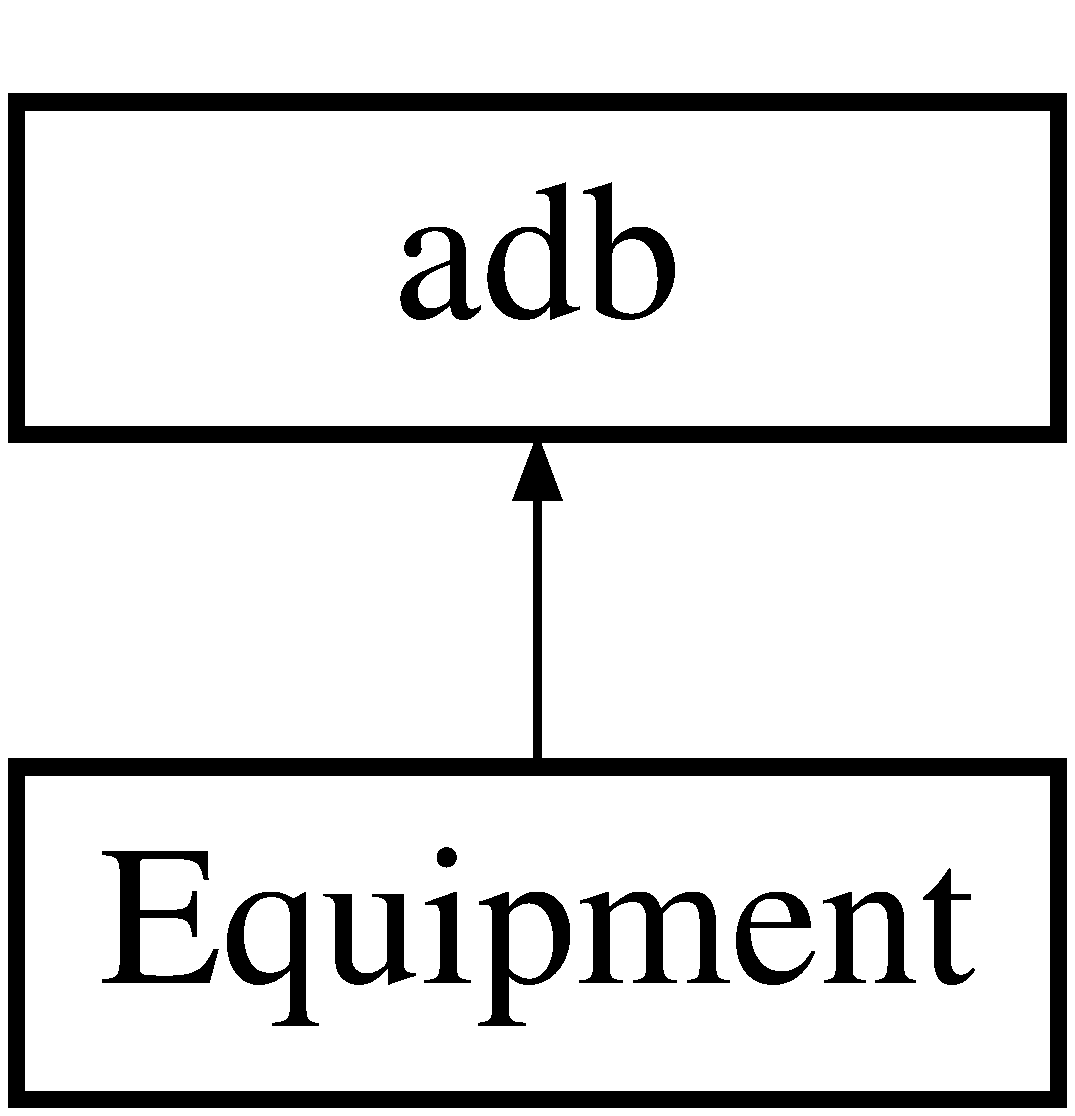
\includegraphics[height=2.000000cm]{class_equipment}
\end{center}
\end{figure}
\subsection*{Public Member Functions}
\begin{DoxyCompactItemize}
\item 
{\bfseries Equipment} ()\hypertarget{class_equipment_a81f0201350767d4c312eb52edc72e397}{}\label{class_equipment_a81f0201350767d4c312eb52edc72e397}

\item 
\hyperlink{class_equipment_a25772ef2833dfcccf9b6dbf4aadbb115}{get\+Tools} (\$filter=false)
\item 
\hyperlink{class_equipment_a560107106e055caba491bd31b8ff4682}{search\+Tool} (\$text=false)
\end{DoxyCompactItemize}
\subsection*{Additional Inherited Members}


\subsection{Detailed Description}
\hyperlink{class_equipment}{Equipment} class 

Definition at line 11 of file Equipment.\+php.



\subsection{Member Function Documentation}
\index{Equipment@{Equipment}!get\+Tools@{get\+Tools}}
\index{get\+Tools@{get\+Tools}!Equipment@{Equipment}}
\subsubsection[{\texorpdfstring{get\+Tools(\$filter=false)}{getTools($filter=false)}}]{\setlength{\rightskip}{0pt plus 5cm}get\+Tools (
\begin{DoxyParamCaption}
\item[{}]{\$filter = {\ttfamily false}}
\end{DoxyParamCaption}
)}\hypertarget{class_equipment_a25772ef2833dfcccf9b6dbf4aadbb115}{}\label{class_equipment_a25772ef2833dfcccf9b6dbf4aadbb115}
Gets tools based on filter 
\begin{DoxyParams}{Parameters}
{\em string} & mixed condition to filter. If false, then filter will not be applied \\
\hline
\end{DoxyParams}
\begin{DoxyReturn}{Returns}
boolean true if successful, else false 
\end{DoxyReturn}


Definition at line 24 of file Equipment.\+php.

\index{Equipment@{Equipment}!search\+Tool@{search\+Tool}}
\index{search\+Tool@{search\+Tool}!Equipment@{Equipment}}
\subsubsection[{\texorpdfstring{search\+Tool(\$text=false)}{searchTool($text=false)}}]{\setlength{\rightskip}{0pt plus 5cm}search\+Tool (
\begin{DoxyParamCaption}
\item[{}]{\$text = {\ttfamily false}}
\end{DoxyParamCaption}
)}\hypertarget{class_equipment_a560107106e055caba491bd31b8ff4682}{}\label{class_equipment_a560107106e055caba491bd31b8ff4682}
Searches tools based on the filter 
\begin{DoxyParams}{Parameters}
{\em string} & mixed condition to filter. If flase, then filter will not be applied \\
\hline
\end{DoxyParams}
\begin{DoxyReturn}{Returns}
boolean true if successful, else false 
\end{DoxyReturn}


Definition at line 38 of file Equipment.\+php.



The documentation for this class was generated from the following file\+:\begin{DoxyCompactItemize}
\item 
C\+:/xampp/htdocs/projimp1/src/Equipment.\+php\end{DoxyCompactItemize}

%--- End generated contents ---

% Index
\backmatter
\newpage
\phantomsection
\clearemptydoublepage
\addcontentsline{toc}{chapter}{Index}
\printindex

\end{document}
